\chapter{Fazit}
\label{cha:fazit}

\section{Zusammenfassung}

Das Ziel der Abschlussarbeit war die Implementierung einer Software, mit welcher Systemadministratoren sich in Echtzeit über den Status eines administrierten Netzwerkes informieren können. Die Informationsquelle für Abfragen ist die Software Graylog Open, welche Systemprotokolle sämtlicher Geräte in einem Netzwerk zentral sammelt und durchsuchbar macht. Den Administratoren sollte es ermöglicht werden, über eine auf gesprochener Sprache basierende Eingabemöglichkeit Anfragen zu verfassen. Die Aufgabe der zu implementierenden Software ist es, die Informationen aus der über den Messenger Telegram gesendeten Sprachnachricht zu extrahieren und damit eine Anfrage an Graylog zu stellen. Schließlich sollte die Software die Antwort von Graylog ebenfalls in einer Sprachnachricht an den Benutzer zurücksenden. 

Die Implementierung der Software verlief planmäßig, sodass die gestellten Anforderungen erfüllt werden konnten. Während der Entwicklung und bei der Prüfung erster Prototypen fiel auf, dass die nicht-funktionalen Anforderungen Verarbeitungsgeschwindigkeit und Erkennungsgenauigkeit der Spracherkennung an ein Produkt, welches ausschließlich per Sprache bedient werden soll hohe Ansprüche an die Qualität der Implementierung stellen. Durch die Verwendung von asynchronen Funktionen konnte die Verarbeitungsgeschwindigkeit erheblich reduziert werden. Eine weitere Funktion, welche zur Verbesserung der Erkennungsgenauigkeit beigetragen hat, waren die implementierten Aliasdefinitionen. Mit diesen konnte die im Gegensatz zur Transkription von alltäglicher Sprache niedrige Treffergenauigkeit von Fachbegriffen aus dem Bereich der Informatik gut kompensiert werden. 

Auch aus Sicht der IT-Sicherheit bringt die Verwendung des Telegram-Bots Vorteile gegenüber der Verwendung der Graylog Webschnittstelle, sofern der Zugriff von außerhalb des Netzwerks erfolgt. Die Graylog-Instanz sammelt die Systemprotokolle sämtlicher Geräte im Netzwerk und ist damit ein besonders schützenswertes System in einem Firmennetzwerk. Der Zugriff von außerhalb sollte gut abgesichert werden. Es existieren mehrere Möglichkeiten, um webbasierte Systeme aus einem internen Netzwerk über das Internet erreichbar zu machen. Eine simple Möglichkeit besteht darin, auf dem Internetrouter eine Portweiterleitung einzurichten. Besser ist jedoch eine Veröffentlichung über einen 'Reverse Proxy'. Ein Proxy ist ein System, welches stellvertretend für ein weiteres System eine Kommunikation mit dem gewünschten Partner übernimmt. Häufig werden Proxys in Firmennetzwerken für die Filterung von besuchten Internetseiten eingesetzt. Dabei wendet sich ein PC im internen Netzwerk an den Proxyserver und fragt eine Internetressource an. Der Proxy agiert als Vermittler und bezieht die Internetressource, bevor er diese an den PC weiterleitet. Bei einem Reverse Proxy ist das Prinzip umgekehrt. Hier übernimmt der Vermittler die Kommunikation von Geräten außerhalb eines Netzwerks (beispielsweise dem Internet) stellvertretend für die Quelle und kontaktiert den gewünschten Verbindungspartner im internen Netzwerk. Der Vorteil eines Reverse Proxys gegenüber einer Portweiterleitung besteht darin, dass die HTTP-Anfragen detailliert bearbeitet, gefiltert und protokolliert werden können. Bestimmte Adressmuster, welche für Angriffe verwendet werden können so beispielsweise direkt blockiert werden. Der alleinige Einsatz eines Reverse Proxys mit Filter für die Veröffentlichung über das Internet reicht bei einem schützenswerten System nicht aus. Daher wird häufig eine HTTP-Authentifizierung zwischengeschaltet, welche durch die Anforderung von vom Ziel unabhängigen Zugangsdaten eine zusätzliche Sicherheitsebene schafft. Ein Reverse Proxy mit auf die Zielapplikation abgestimmten Filtermechanismen sowie einer zusätzlichen Authentifizierungsschicht bietet ausreichenden Schutz für eine Veröffentlichung im Internet. Der Einsatz eines solchen Reverse Proxies mit Graylog ist jedoch nicht möglich, da Graylog nicht kompatibel zu Anfragen mit HTTP-Authentifizierung ist \footnote{Fehlerbericht und Erweiterungsvorschlag eines Anwenders, welcher Graylog über einen Reverse Proxy mit HTTP-Authentifizierung erreichbar machen möchte: \url{https://github.com/Graylog2/graylog2-server/issues/6831}}. Eine Alternative zum Reverse Proxy bietet ein Dienst, welcher die Funktion eines Proxys oder Stellvertreters für die Verbindung zur Graylog-Webschnittstelle schafft. Dieser Dienst kann für beliebige Funktionen implementiert werden, welche über die Graylog REST-API Daten beziehen und weiterverarbeiten. Die in dieser Abschlussarbeit implementierte Software ist ein Beispiel für einen solchen Vermittler auf Applikationsebene (vgl. Empfehlungen des BSI zur Absicherung von Webangeboten \cite[S. 12 ff.]{bsi-websec}).

\section{Anwendung}

Der Code der entwickelten Software wurde über ein GitHub-Repository \footnote{\url{https://github.com/Jomibe/ba}} veröffentlicht, sodass die Installation und Konfiguration des Bots für eine eigene Installation von Graylog wiederverwendet oder optimiert werden kann. Für den Betrieb ist es notwendig, zuvor die angeschlossenen Dienste inkl. der API-Zugriffsdaten zu konfigurieren. Im Anschluss kann die Software mit einem Python Interpreter ausgeführt werden und ist einsatzbereit, sobald die Vorbereitungsphase abgeschlossen ist. Mithilfe der aktivierten ausführlichen Ausgaben zum Programmablauf können die Vorgänge und dessen Auslöser gut zurückverfolgt werden. Im Folgenden zeigen zwei Abbildungen die Interaktion mit dem Bot über den Telegram Messenger:

\begin{figure}[h!]
    \centering
    \begin{minipage}{0.5\textwidth}
        \raggedright
        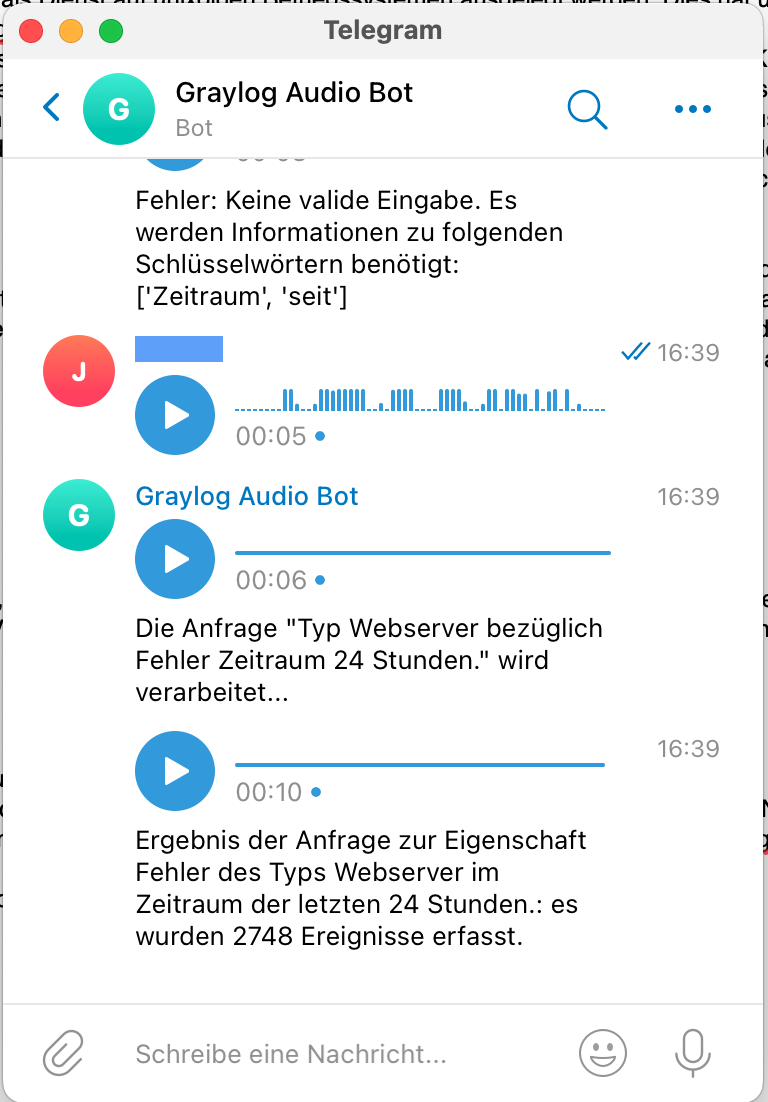
\includegraphics[width=0.9\textwidth]{bsp-betrieb}
        \caption{Bot beantwortet eine \\\hspace{\textwidth}Anfrage in Telegram.}
        \label{fig:bsp-betrieb}
    \end{minipage}\hfill
    \begin{minipage}{0.5\textwidth}
        \raggedleft
        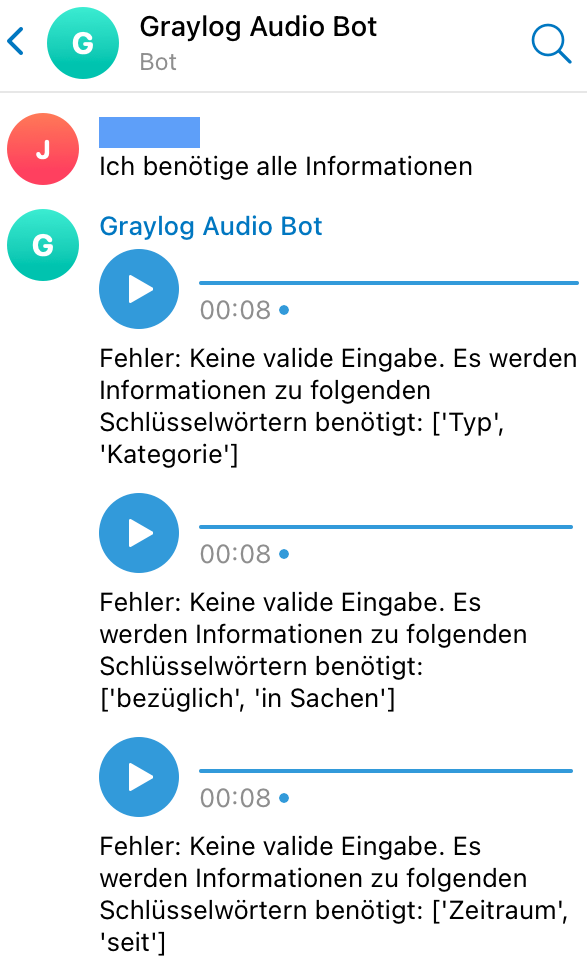
\includegraphics[width=0.9\textwidth]{bsp-fehler}
        \caption{Bot reagiert auf fehlerhafte \\\hspace{\textwidth}Anfrage in Telegram.}
        \label{fig:bsp-fehler}
    \end{minipage}
\end{figure}

Die obige Abbildung zeigt, wie der Bot eine Anfrage beantwortet. Zuerst wird dem Benutzer eine Rückmeldung gesendet, sobald die Transkription fertiggestellt ist. Im Anschluss erfolgt die Beantwortung der eingesendeten Anfrage. Alle Nachrichten des Bots werden in einer kombinierten Sprachnachricht gesendet, welche zusätzlich den gesprochenen Text in geschriebener Form enthält. Zusätzlich ist es möglich, Anfragen per Textnachricht einzusenden, wie \autoref{fig:bsp-fehler} zeigt:

In \autoref{fig:bsp-fehler} wurde dem Bot eine Nachricht zugestellt, welche nicht die erforderlichen Informationen beinhaltet. Der Bot prüft dies anhand der konfigurierten Schlüsselwörter und weißt den Anwender auf jede fehlende Information hin. 

\subsection{Qualitätskontrolle}

Nach Abschluss der Implementierung soll die Qualität der Software bezüglich der Benutzbarkeit im geplanten Anwendungsfall kurz erläutert werden. Die Qualität der Anwendung hängt stark von der Qualität der Spracherkennung ab, da hiervon die höchste Fehlerwahrscheinlichkeit ausgeht. Mit dem Vergleich verschiedener Dienste (vgl. \autoref{sec:vergleich-transkrip}) konnte dieses Qualitätsmerkmal bereits vor der Implementierung optimiert werden. Durch die Möglichkeit, Anfragen ebenfalls als Textnachricht an die Software zu übermitteln, kann der Anwender die Fehlerwahrscheinlichkeit bei der Erkennung des Anliegens reduzieren. Weiterhin ist es möglich, lokale Transkriptionsdienste, beispielsweise von der Tastatur-App auf einem Mobiltelefon zu nutzen. Ein weiteres Werkzeug für die Verbesserung der Spracherkennung sind die Aliasdefinitionen. Der Vergleich der verschiedenen Dienste hat bereits bei einer kleinen Stichprobe gezeigt, dass die Spracherkennung bei Fachbegriffen nicht verlässlich genug arbeitet. Die Definition von Begriffen aus der Alltagssprache als Alias für Fachbegriffe führt daher zu einer Verbesserung der Erkennungsquote und somit zu einem gesteigerten Qualitätsempfinden der Anwendung aus Sicht der Benutzer.

\section{Ausblick}

Es sind einige Erweiterungen der Funktionalität der entwickelten Software denkbar. 

\subsection{Nebenläufigkeit}

Die ersten Voraussetzungen für eine vollständige Nebenläufigkeit von Prozessen wurden bereits mit der Verwendung des Amazon Transcribe SDK erfüllt. Derzeit verarbeitet der Bot die eingehenden Nachrichten synchron, bzw. nacheinander. Es ist jederzeit möglich, neue Nachrichten einzusenden, diese werden jedoch sequenziell statt parallel verarbeitet. Um die parallele Verarbeitung von eingehenden Nachrichten zu ermöglichen, ist es notwendig, asynchrone Funktionen auch in weiteren Programmmodulen einzusetzen. Weiterhin ist es denkbar, die Software für den Betrieb mit mehreren Threads oder einem Orchestrierungsdienst wie Kubernetes anzupassen. Anfragen würden dann von einer Softwarekomponente angenommen und auf freie Instanzen verteilt werden, welche die Anfrage durchführen und das Ergebnis asynchron an die Hauptinstanz zurückführen. 

\subsection{Datenaufbereitung}

Derzeit gibt die Software für jede Anfrage die Anzahl der erfassten Ereignisse zurück. Diese Angabe ist nicht für jede Abfrage sinnvoll. Zukünfig könnten weitere Funktionen für die Aufbereitung der Informationen inkl. weiteren Schlüsselwörtern implementiert werden, welche beispielsweise den Minimal- oder Maximalwert oder alle verschiedenen Werte (analog zum SQL Statement \lstinline{SELECT DISTINCT}) ausgeben.

\subsection{Verwaltung per Telegram}

Änderungen am Verhalten der Software und insbesondere an den Zuordnungen der Suchbegriffe zu den Schlüsselwörtern können derzeit nur über eine Anpassung von Konfigurationsdateien vorgenommen werden. In Zukunft könnte ein Rollenkonzept eingeführt werden, welches es bestimmten Benutzern erlaubt, Änderungen an den Zuordnungen vornehmen zu dürfen und neue Abfragen definieren zu können.
